\documentclass[12pt, a4paper]{article}
\usepackage[T1]{fontenc}
\usepackage[utf8]{inputenc}
\usepackage[brazilian]{babel}
\usepackage{times}
\usepackage[top=3cm, bottom=2cm, left=3cm, right=2cm]{geometry}
\usepackage{setspace}
\usepackage{indentfirst}
\usepackage{titlesec}
\usepackage{hyperref}

% ABNT: títulos de seções em maiúsculas, negrito, 12pt
\titleformat{\section}{\normalfont\bfseries\uppercase}{\thesection}{1em}{}
\titleformat{\subsection}{\normalfont\bfseries}{\thesubsection}{1em}{}

\begin{document}

% -------------------------------------------------------
% CAPA (ABNT NBR 14724)
% -------------------------------------------------------
\begin{titlepage}
    \begin{center}
        {\normalsize\bfseries INSTITUTO FEDERAL DE EDUCAÇÃO, CIÊNCIA E TECNOLOGIA DO RIO GRANDE DO NORTE}

        \vfill

        {\normalsize\bfseries JHONATA SANTANA FERREIRA}

        \vfill

        {\normalsize\bfseries DESAFIOS E OPORTUNIDADES NO DESENVOLVIMENTO DE UM JOGO PARA O CAMPUS: DESBRAVANDO O CAMPUS}

        \vfill

        {\normalsize PARNAMIRIM-RN}\\[0.3cm]
        {\normalsize 2026}
    \end{center}
\end{titlepage}

% -------------------------------------------------------
% FOLHA DE ROSTO (ABNT NBR 14724)
% -------------------------------------------------------
\begin{titlepage}
    \begin{center}
        {\normalsize\bfseries JHONATA SANTANA FERREIRA}

        \vfill

        {\normalsize\bfseries DESAFIOS E OPORTUNIDADES NO DESENVOLVIMENTO DE UM JOGO PARA O CAMPUS: DESBRAVANDO O CAMPUS}
    \end{center}

    \vfill

    \begin{flushright}
        \begin{minipage}{0.5\textwidth}
            \normalsize
            Relatório apresentado ao Curso Tecnólogo em Sistemas para Internet, na disciplina de  Seminário de Orientação ao Trabalho de Conclusão de Curso,
            no Instituto Federal de Educação, Ciência e Tecnologia do Rio Grande do Norte, como requisito parcial de avaliação.
            
            \vspace{0.8cm}
            Orientador: A DEFINIR
        \end{minipage}
    \end{flushright}

    \vfill

    \begin{center}
        {\normalsize PARNAMIRIM-RN}\\[0.3cm]
        {\normalsize 2026}
    \end{center}
\end{titlepage}

% -------------------------------------------------------
% CONFIGURAÇÕES PÓS-CAPA
% -------------------------------------------------------
\setcounter{page}{1}         % numeração começa após as capas
\onehalfspacing              % espaçamento 1,5 (ABNT)
\setlength{\parindent}{1.25cm} % recuo de parágrafo (ABNT)

% -------------------------------------------------------
% SEÇÕES
% -------------------------------------------------------

\newcommand{\assinatura}[1]{%
    \vspace{1.3cm}
    \begin{center}
        \rule{0.85\textwidth}{0.4pt}\\[-2pt]
        {\normalsize #1}\\[-2pt]
        {\footnotesize Instituto Federal de Educação, Ciência e Tecnologia do Rio Grande do Norte}
    \end{center}
}

% ===== FOLHA DE ROSTO =====
\begin{titlepage}
    \begin{center}
        {\normalsize\bfseries JHONATA SANTANA FERREIRA}

        \vfill

        {\normalsize\bfseries DESAFIOS E OPORTUNIDADES NO DESENVOLVIMENTO DE UM JOGO PARA O CAMPUS: DESBRAVANDO O CAMPUS}
    \end{center}

    \vfill

    \begin{flushright}
        \begin{minipage}{0.5\textwidth}
            \normalsize
            \setlength{\parindent}{0pt}
            Relatório apresentado ao Curso Tecnólogo em Sistemas para Internet, na disciplina de Seminário de Orientação ao Trabalho de Conclusão de Curso, no Instituto Federal de Educação, Ciência e Tecnologia do Rio Grande do Norte, como requisito parcial de avaliação.

            \vspace{0.5cm}
            Orientador: A DEFINIR
        \end{minipage}
    \end{flushright}

    \vfill

    \begin{center}
        {\normalsize PARNAMIRIM-RN}\\[0.3cm]
        {\normalsize 2026}
    \end{center}
\end{titlepage}

% ===== FOLHA DE APROVAÇÃO =====
\begin{titlepage}
    \begin{center}
        {\normalsize\bfseries JHONATA SANTANA FERREIRA}

        \vspace{1.5cm}

        {\normalsize\bfseries DESAFIOS E OPORTUNIDADES NO DESENVOLVIMENTO DE UM JOGO PARA O CAMPUS: DESBRAVANDO O CAMPUS}
    \end{center}

    \vspace{1cm}

    \begin{flushright}
        \begin{minipage}{0.5\textwidth}
            \normalsize
            \setlength{\parindent}{0pt}
            Relatório apresentado ao Curso Tecnólogo em Sistemas para Internet, na disciplina de Seminário de Orientação ao Trabalho de Conclusão de Curso, no Instituto Federal de Educação, Ciência e Tecnologia do Rio Grande do Norte, como requisito parcial de avaliação.
        \end{minipage}
    \end{flushright}

    \vspace{1cm}

    \noindent Aprovado em: \underline{\hspace{0.8cm}}/\underline{\hspace{0.8cm}}/\underline{\hspace{1.2cm}}

    \vspace{0.8cm}
    \begin{center}
        Banca Examinadora
    \end{center}

    \assinatura{A definir -- Orientador}
    \assinatura{-- Examinador}
    \assinatura{-- Examinador}
\end{titlepage}

\newpage

\tableofcontents
\newpage

\section{INTRODUÇÃO}

O presente relatório descreve a inspiração e motivação para a criação do jogo
lúdico \textit{Desbravando o Campus}, desenvolvido com o motor gráfico
\textit{Unity} e os conceitos de Programação Orientada a Objetos (POO).
Para manter o \textit{game} atualizado, será utilizado um ambiente Docker
com integração contínua (CI) para atualizações do jogo e de sua \textit{landing page}.

\bigbreak

O Instituto Federal de Educação, Ciência e Tecnologia do Rio Grande do Norte
(\textit{IFRN}), por meio do Curso Superior de Tecnologia em Sistemas para Internet
do \textit{campus} Parnamirim, busca integrar tecnologias e inovações emergentes em
sua grade curricular, proporcionando aos estudantes experiências práticas que os
preparem para os desafios do mercado de trabalho. O \textit{Desbravando o Campus}
surge nesse contexto como projeto de conclusão de curso, permitindo que calouros e
visitantes conheçam virtualmente a estrutura do \textit{campus} Parnamirim e a rotina
de seus estudantes e colaboradores.


\subsection{Inspiração}

A inspiração para a criação do \textit{game} foi o popular jogo de gênero
\textit{top-down} denominado \textit{Stardew Valley}. Esse título foi escolhido
por ser acolhedor, lúdico e visualmente confortável, transmitindo segurança e
empatia ao jogador. Tais características se alinham diretamente ao propósito do
\textit{Desbravando o Campus}: acolher calouros e visitantes que desconhecem a
estrutura e o funcionamento do \textit{campus}.

\subsection{Problema da Pesquisa}

O problema que este projeto de conclusão aborda é relevante para a comunidade acadêmica.
Suponha que um estudante recém-aprovado em um dos cursos do \textit{IFRN} desconheça
a estrutura do \textit{campus} e seu funcionamento. O \textit{Desbravando o Campus}
surge como um suporte acolhedor a novos estudantes e visitantes em geral, oferecendo
uma forma de explorar e conhecer o \textit{campus} sem a necessidade de presença física.

Isso pode impactar positivamente estudantes introvertidos, que muitas vezes enfrentam
pressão social ao precisar conhecer um novo ambiente desacompanhados. Caso o calouro
ou visitante não possua nenhum contato prévio no \textit{campus}, o jogo oferece uma
alternativa acessível e sem julgamentos para essa primeira aproximação.

\newpage

\subsection{Justificativa e Relevância}

O desenvolvimento do \textit{Desbravando o Campus} justifica-se por um conjunto de fatores
bem presente na realidade de todos os \textit{campus}:

\bigbreak

{\bfseries Justificativa Técnica:} O desenvolvimento do \textit{Desbravando o Campus} foi realizado com o motor gráfico
\textit{Unity}, amplamente utilizado na indústria de jogos digitais e reconhecido por
sua versatilidade no desenvolvimento de aplicações 2D e 3D. A escolha do \textit{Unity}
se justifica pela sua extensa documentação, comunidade ativa e suporte nativo à linguagem
C\#, que possibilita a aplicação direta dos conceitos de Programação Orientada a Objetos
(POO) trabalhados ao longo do curso.

A arquitetura do projeto adota o padrão de projeto \textit{Component-Based Architecture},
nativo do \textit{Unity}, no qual cada entidade do jogo é composta por componentes
independentes e reutilizáveis. Essa abordagem favorece a manutenibilidade e a escalabilidade
do código, princípios fundamentais no desenvolvimento de software.

Para garantir a continuidade e a atualização do jogo, foi adotada uma esteira de
integração contínua (CI/CD) com Docker, permitindo que novas versões sejam entregues
de forma automatizada e controlada. O versionamento do código é gerenciado via
\textit{Git}, com repositório hospedado no \textit{GitHub}, assegurando rastreabilidade
e controle das alterações realizadas ao longo do desenvolvimento.

\bigbreak

{\bfseries Justificativa Educacional:} O projeto serve como ambiente de aprendizagem
prático, no qual são aplicados componentes da grade curricular do curso de forma
integrada. Além disso, proporciona uma experiência diferenciada para calouros e
visitantes do \textit{campus}, oferecendo suporte àqueles que não dispõem de contatos
prévios para auxiliá-los na adaptação ao novo ambiente acadêmico. O
\textit{Desbravando o Campus} surge, portanto, como uma alternativa acessível e
inclusiva para suprir essa necessidade.

\subsection{Objetivos}

\subsubsection{Objetivo Geral}

Desenvolver um jogo do Instituto Federal de Educação, Ciência e Tecnologia \textit{(IFRN)},
para aprofundar nas disciplina de Programação Orientada a Objetos\textit{ (POO)}, Padrões de projetos\textit{(UML)}, 
Desenvolvimento em Nuvem\textit{ (CI/CD)}. Para ajudar os estudantes calouros e visitantes conhecerem a estrutura do 
\textit{campus}, quanto sua rotina e alguns colaboradores presente na instituição de ensino. 

\newpage

\subsubsection{Objetivo Específicos}

\begin{itemize}
    \item Modelar a arquitetura do sistema utilizando a Linguagem de Modelagem
    Unificada (UML), contemplando diagramas de classes, casos de uso e sequência;

    \item Implementar o jogo utilizando o motor gráfico \textit{Unity} e a linguagem
    C\#, aplicando os princípios de Programação Orientada a Objetos (POO);

    \item Estruturar o projeto com o padrão \textit{Component-Based Architecture},
    garantindo modularidade, manutenibilidade e escalabilidade do código;

    \item Configurar uma esteira de integração e entrega contínua (CI/CD) com
    \textit{Docker}, automatizando o processo de build e deploy do jogo;

    \item Desenvolver uma \textit{landing page} para divulgação e distribuição
    do jogo ao público-alvo;

    \item Avaliar a experiência dos usuários por meio de testes com calouros e
    visitantes do \textit{campus} Parnamirim.
\end{itemize}

% =======================================================
% METODOLOGIA - TRILHA 3: DESENVOLVIMENTO DE UMA SOLUÇÃO TECNOLÓGICA
% Pacote necessário (se for inserir as figuras): \usepackage{graphicx}
% =======================================================

\newpage

\section{METODOLOGIA}

Esta seção descreve o ciclo de desenvolvimento do \textit{Desbravando o Campus},
organizado em quatro etapas: levantamento de requisitos, especificação da solução,
plano de implementação e realização de testes.

\subsection{Levantamento de Requisitos}

Os requisitos foram elicitados a partir do problema de pesquisa e do público-alvo
do projeto (calouros e visitantes do \textit{campus} Parnamirim), considerando
a inspiração no gênero \textit{top-down} e a necessidade de uma experiência
acolhedora e sem pressão social.

\subsubsection{Requisitos Funcionais}

\begin{itemize}
    \item \textbf{RF01:} o jogador deve movimentar o personagem nas quatro direções
    por meio do teclado;

    \item \textbf{RF02:} o personagem deve exibir animações de caminhada e de
    repouso de acordo com a última direção percorrida;

    \item \textbf{RF03:} o jogo deve representar virtualmente os ambientes do
    \textit{campus}, respeitando colisões com paredes e objetos;

    \item \textbf{RF04:} o jogador deve poder interagir com personagens que
    representam colaboradores da instituição;

    \item \textbf{RF05:} o jogo deve apresentar informações sobre os espaços do
    \textit{campus} e sobre a rotina de estudantes e colaboradores;

    \item \textbf{RF06:} a \textit{landing page} deve permitir ao usuário conhecer
    o projeto e obter a versão atual do jogo.
\end{itemize}

\subsubsection{Requisitos Não Funcionais}

\begin{itemize}
    \item \textbf{RNF01 (Usabilidade):} os controles devem ser simples e
    compreensíveis por usuários sem experiência prévia com jogos;

    \item \textbf{RNF02 (Desempenho):} o jogo deve manter taxa de quadros estável
    em computadores de configuração intermediária;

    \item \textbf{RNF03 (Manutenibilidade):} o código deve seguir a arquitetura
    baseada em componentes e os princípios de POO, com classes de responsabilidade
    única;

    \item \textbf{RNF04 (Portabilidade):} a distribuição deve funcionar nos
    sistemas operacionais e navegadores mais comuns entre o público-alvo;

    \item \textbf{RNF05 (Atualização):} novas versões devem ser geradas e
    publicadas de forma automatizada, por meio de CI/CD.
\end{itemize}

\subsection{Especificação da Solução}

\subsubsection{Casos de Uso}

O sistema possui dois atores: o \textbf{Jogador} (calouro ou visitante) e o
\textbf{Desenvolvedor}, responsável por publicar novas versões. Os principais
casos de uso são descritos a seguir.

\begin{itemize}
    \item \textbf{UC01 -- Explorar o \textit{campus}:} o jogador move o personagem
    pelo mapa. \textit{Fluxo principal:} o jogador pressiona as teclas de direção;
    o sistema lê a entrada, desloca o personagem e atualiza a animação. 
    \textit{Pré-condição:} jogo iniciado.

    \item \textbf{UC02 -- Interagir com colaborador:} o jogador se aproxima de
    um personagem e inicia uma conversa para conhecer sua função na instituição.

    \item \textbf{UC03 -- Consultar informações dos espaços:} o jogador acessa
    informações sobre os ambientes visitados e sobre a rotina do \textit{campus}.

    \item \textbf{UC04 -- Obter o jogo:} o jogador acessa a \textit{landing page}
    e baixa a versão mais recente.

    \item \textbf{UC05 -- Publicar nova versão:} o desenvolvedor envia o código
    ao repositório; a esteira de CI/CD gera o \textit{build} e atualiza o jogo e a
    \textit{landing page}.
\end{itemize}

\begin{figure}[h]
    \centering
    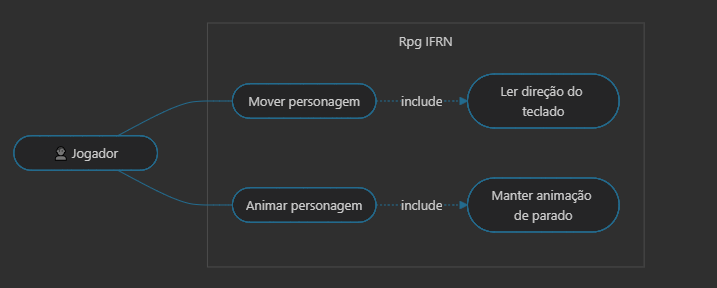
\includegraphics[width=0.9\textwidth]{../Docs/Images/use_case.png}
    \caption{Diagrama de casos de uso do \textit{Desbravando o Campus}}
\end{figure}

\subsubsection{Modelagem Arquitetural}

A arquitetura segue o padrão \textit{Component-Based Architecture} do
\textit{Unity}, no qual cada entidade é composta por componentes independentes.
O personagem, por exemplo, é formado pela classe \texttt{PlayerIFRN}, que lê o
teclado e movimenta o \texttt{Rigidbody2D}, e pela classe \texttt{PlayerAnimIFRN},
que consulta a direção do jogador e define o parâmetro \texttt{Transition} do
\texttt{Animator}. Assim, a lógica de movimento e a de animação permanecem
separadas, e cada uma pode ser alterada sem afetar a outra.

O fluxo de dados do jogo é: entrada do teclado $\rightarrow$ \texttt{PlayerIFRN}
$\rightarrow$ propriedade \texttt{direction} $\rightarrow$ \texttt{PlayerAnimIFRN}
$\rightarrow$ \texttt{Animator}. Já o fluxo de entrega é: repositório
\textit{GitHub} $\rightarrow$ esteira de CI/CD em \textit{Docker} $\rightarrow$
\textit{build} do jogo $\rightarrow$ \textit{landing page}. Na versão atual, o
jogo não depende de banco de dados nem de APIs externas.


\begin{figure}[h]
    \centering
    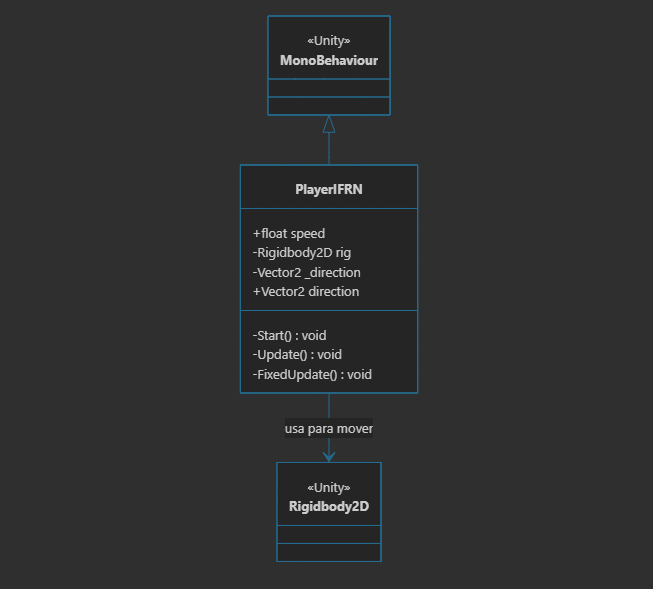
\includegraphics[height=0.45\textheight]{../Docs/Images/class_diagram_PlayerIFRN.png}
    \caption{Diagrama de classes do personagem jogável}
\end{figure}

\subsection{Plano de Implementação}

\subsubsection{Tecnologias Adotadas}

\begin{itemize}
    \item \textbf{Motor gráfico e linguagem:} \textit{Unity} e C\#, aplicando
    POO;

    \item \textbf{Recursos visuais:} \textit{sprites} e \textit{tilesets} 2D para
    a ambientação do \textit{campus}, com \textit{NavMeshPlus} para a navegação de
    personagens não jogáveis;

    \item \textbf{Versionamento:} \textit{Git}, com repositório no \textit{GitHub};

    \item \textbf{Containers e CI/CD:} \textit{Docker}, para padronizar o ambiente
    de \textit{build} e automatizar a entrega;

    \item \textbf{\textit{Front-end} de divulgação:} \textit{landing page} com
    HTML, CSS e JavaScript;

    \item \textbf{Modelagem:} UML e \textit{Mermaid}, com documentação organizada
    em um diretório \texttt{Docs}, fora da pasta \texttt{Assets} do \textit{Unity}.
\end{itemize}

\subsubsection{Protótipos de Interface}

Serão elaborados protótipos (\textit{mockups}) das telas principais: menu inicial,
cenário de exploração, caixa de diálogo com colaboradores e \textit{landing page}.
Os protótipos serão validados antes da implementação final, de modo a priorizar
legibilidade e simplicidade, em consonância com o requisito RNF01.

\subsection{Realização de Testes}

Os testes serão realizados em quatro frentes:

\begin{itemize}
    \item \textbf{Testes de navegação:} percorrer todo o mapa nas quatro direções,
    verificando colisões, limites do cenário e ausência de áreas inacessíveis;

    \item \textbf{Testes funcionais:} verificar cada requisito funcional por meio
    de roteiros. Por exemplo, para o RF02, conferir se a animação de repouso
    corresponde à última direção percorrida;

    \item \textbf{Compatibilidade de dispositivos:} executar o jogo e acessar a
    \textit{landing page} em diferentes resoluções, sistemas operacionais e
    navegadores;

    \item \textbf{Testes de usabilidade:} aplicar o jogo a um grupo de calouros e
    visitantes do \textit{campus} Parnamirim, com observação da navegação e
    questionário de satisfação, a exemplo da escala \textit{System Usability Scale}
    (SUS).
\end{itemize}

Cada teste terá um roteiro com o objetivo, os passos, o resultado esperado e o
resultado obtido. Os problemas encontrados serão registrados e corrigidos antes
da publicação da versão final.


\end{document}